\chapter{Especificación de requisitos}


\section{Introducción}
En esta sección se describirá qué vamos a construir y cómo lo vamos a hacer, 
con sus restricciones específicas. Esto se realizará especificando y describiendo
 detallar los requisitos del sistema que vamos a desarrollar. 

\subsection{Propósito}
En este capítulo se pretende describir de forma clara y precisa las funciones, carasterísticas y restricciones
del sistema que se va a desarrollar. Estas definiciones servirán al equipo de desarrolo para
conocer las necesidades del sistema y a los usuarios finales. Además, este documento será será consultado como
base para el desarrollo de las funcionalidades descritas en la sección de implementación.

\subsection{Ámbito del Sistema}
El sistema que vamos a desarrollar es una aplicación multiplataforma llamada "Meloudy" que permitirá a los usuarios
aprender conceptos musicales de una forma amena, fácil y divertida. Esto se logrará mediante el método de gamificación,
utilizando un sistema de logros y de recompensas con la superación de los distintos ejercicios y actividades de distintos tipos que el usuario deberá completar.
Además, la aplicación llevará el progreso de los usuarios que les permitirá saber cómo van en su aprendizaje.

\subsection{Definiciones, Acrónimos y Abreviaturas}
A continuación se detallará el significado de algunos conceptos importantes para la comprensión del documento y de nuestro sistema.
\begin{itemize}
    \item \textbf{Requisito:} Es una condición o característica que debe cumplir el sistema para satisfacer una necesidad o cumplir una función.
    \item \textbf{Funcionalidad:} Descripción de lo que debe hacer el producto software.
    \item \textbf{Restricción:} Condición que limita la funcionalidad del sistema.
    \item \textbf{Interfaces externas:} Tipo de requisito que incluye la interfaz de usuario (interacción entre el software y el usuario), los diseños de pantallas, las interfaces hardware y software, etc.
    \item \textbf{Usuario: }Persona que utilizará la aplicación para la intención final de esta.
    \item \textbf{Administrador: } Persona encargada del sistema software y del mantenimiento de este para su buen funcionamiento.
    \item \textbf{RF / RNF:} Requisito funcional / Requisito No Funcional.
\end{itemize}

\subsection{Referencias}
Esta sección de Especificación de requisitos ha sido redactada consultando los documentos del estándar IEEE Recommended Practice for Software Requirements Specification ANSI/IEEE 830, 1998.

\subsection{Visión General del Documento}
El documento consta de tres partes bien diferenciadas:
\begin{itemize}
    \item \textbf{Introducción:} Proporciona una visión general sobre el apartado de Especificación de Requisitos sin profundizar en los requisitos como tal.
    \item \textbf{Descripción General:} Se describirá el sistema a construir para saber las funciones principales, los datos necesarios, las restricciones y otros aspectos que puedan afectar al desarrollo de la aplicación.
    \item \textbf{Requisitos Específicos:} Se profundiza en las necesidades del usuario definiendo los requisitos que debe tener nuestro sistema tras el desarrollo y la implementación de este.
\end{itemize}

\section{Descripción General}
A continuación, se procederá a describir con poco detalle los requisitos del sistema de una forma general para saber las funciones principales a desarrollar, las características de los usuarios, las dependencias, etc.
\subsection{Perspectiva del producto}
Se pretende implementar un sistema que permita el aprendizaje del usuario mediante técnicas de gamificación y ejercicios a resolver. Algunas de estas actividades utilizarán librerías para la detección de notas musicales
a partir de la frecuencia captada por el micrófono del usuario y, por tanto, la aplicación dependerá de dichas librerías que se incluyan.
Por otro lado, el sistema de administración y el progreso de los usuarios se llevará a cabo utilizando una base de datos en la que se almacenará la información necesaria de los usuarios y su progreso.

La interacción de los usuarios con la aplicación será mediante una interfaz gráfica que podrá ser utilizada con la pantalla táctil o el ratón del dispositivo usado.

\subsection{Funciones del producto}
Las principales funciones que el usuario podrá realizar dentro de la aplicación son:
\begin{itemize}
\item Selección de lecciones a aprender.
\item Respuesta (mediante selección o escritura) de las preguntas y actividades que ofrezca la aplicación.
\item Consulta del progreso individual, de los logros obtenidos y de la clasifiación global.
\item Modificación de los datos del perfil.
\end {itemize}

Además, el encargado/profesor se encargará de parte de la administración de las lecciones mediante:
\begin{itemize}
    \item Modificación y creación del texto de la lección
    \item Modificación de las preguntas y actividades
    \item Creación de preguntas para una lección
\end{itemize}

\subsection{Características de los usuarios}
Los usuarios que usarán la aplicación tendrán distintos perfiles y abarcarán edades muy distintas. Aún así,
el perfil objetivo para el uso del sistema será las personas jóvenes, pues suelen utilizar mucho más las nuevas tecnologías
y estarán más familiarizados con este tipo de aplicaciones. No se necesita conocimiento musical previo para utilizar el software y,
de hecho, las lecciones pueden ser bastante básicas y sencillas para las personas que ya conozcan conceptos y aspectos avanzados del lenguaje musical.


\subsection{Restricciones}

Las restricciones del sistema a desarrollar son:
\begin{itemize}
    \item La aplicación del cliente estará desarrollada en Flutter y/o Dart y para la del servidor se utilizará NodeJS con Express.
    \item Se utilizarán las consultas, inserciones, modificaciones y borrados de MongoDB para la base de datos, usando un modelo no relacional.
    \item Al hacer uso de librerías externas para desarrollar algunas de las funciones, el rendimiento y las limitaciones hardware pueden depender de estas.
    \item No se podrá registrar un usuario en la aplicación con un correo o nombre de usuario ya existente.
    \item Para completar una lección, el usuario deberá pasar por la pantalla del temario y de los ejercicios, respondiendo a estos.
\end{itemize}


Además, es posible que el sistema tenga que adaptarse a los cambios del entorno y necesite agregar con el paso del tiempo funcionalidades que añadan valor
al producto.


\subsection{Suposiciones y dependencias}
Los requisitos especificados en este documento pueden estar sujetos a cambios por motivos técnicos, de alcance o de refinamiento por la necesidad de la adaptación
al entorno y a la evolución continua del proyecto.

No habrá ningúna suposición respecto al sistema operativo a utilizar puesto que pretendemos desarrollar una aplicación multiplataforma, aunque se priorizará el buen funcionamiento en Android y en navegadores web.

Asumiremos también que las bibliotecas a utilizar para el desarrollo de ciertos requisitos funcionan correctamente y son estables.

\subsection{Futuros requisitos}
Puesto que el entorno puede ser cambiante, el sistema deberá adaptarse a los cambios y a las nuevas necesidades para los usuarios que surjan.
Por tanto, es posible que se añadan nuevos requisitos cuando se modifiquen o añadan funcionalidades al software.

\section{Requisitos Específicos}
A continuación se listarán todos los requisitos que debe cumplir el sistema a desarrollar. Se dividirán en distintos tipos en función de sus objetivos.

\subsection{Requisitos funcionales}
En esta sección se presentan los requisitos relacionados con las funcionalidades del sistema y su comportamiento, sus servicios y las tareas que este debe realizar.

\begin{itemize}
    \item \textbf{General}
          \begin{itemize}
              \item \textbf{RF 1 - Registro de usuarios: }Los usuarios deberán registrarse en el sistema para utilizar la funcionalidad de la aplicación.
              \item \textbf{RF 2 - Identificar usuarios: }Los usuarios deberán identificarse en el sistema con su cuenta para poder utilizar la funcionalidad de la aplicación.

          \end{itemize}
    \item \textbf{Usuarios}
          \begin{itemize}
              \item \textbf{RF 3 - Consultar datos de la cuenta: }Los usuarios podrán consultar los datos de su perfil.
              \item \textbf{RF 4 - Modificar datos de la cuenta: }Los usuarios podrán modificar los datos de su perfil (imagen de perfil, nombre, contraseña...).
              \item \textbf{RF 5 - Selección de lección: }Los usuarios podrán seleccionar la lección a estudiar de la lista de lecciones de la pantalla principal.
              \item \textbf{RF 6 - Responder preguntas: }Los usuarios podrán responder las preguntas de cada tipo en la lección que estén.
                    \begin{itemize}
                        \item \textbf{RF 6.1 - Responder con texto: }Los usuarios podrán responder preguntas que necesiten insertar texto como respuesta.
                        \item \textbf{RF 6.2 - Responder seleccionando una opción: }Los usuarios podrán responder preguntas que necesiten seleccionar una opción de varias que hay.
                        \item \textbf{RF 6.3 - Responder tocando una nota: }Los usuarios podrán responder preguntas que necesiten toca una nota de un instrumento y captarla por el micrófono.
                    \end{itemize}

              \item \textbf{RF7 - Consultar ranking: }Los usuarios podrán consultar la clasificación global de los usuarios.
              \item \textbf{RF8 - Consultar progreso: } Los usuarios podrán consultar su progreso y sus logros obtenidos en su perfil.
          \end{itemize}
    \item \textbf{Profesores/Encargados}
          \begin{itemize}
              \item \textbf{RF 9 - Obtener lista de lecciones: } Los profesores podrán obtener una lista de todas las lecciones que existen en el sistema.
              \item \textbf{RF 10 - Crear lección: }Los profesores podrán crear nuevas lecciones.
              \item \textbf{RF 11 - Modificar temarios: }Los profesores podrán modificar el texto y las imágenes de los temarios de las distintas lecciones.
              \item \textbf{RF 12 - Crear preguntas: } Los profesores podrán crear nuevas preguntas sobre las disintas lecciones
              \item \textbf{RF 13 - Obtener lista de preguntas: } Los profesores podrán obtener una lista de todas las preguntas que existen en el sistema.
              \item \textbf{RF 14 - Modificar preguntas: } Los profesores podrán modificar preguntas ya creadas.
              \item \textbf{RF 15 - Eliminar preguntas: } Los profesores podrán eliminar preguntas del sistema.
          \end{itemize}
    \item \textbf{Administradores}
          \begin{itemize}
              \item \textbf{RF 16 - Modificar datos de usuarios: }Los administradores podrán modificar los datos de un usuario
              \item \textbf{RF 17 - Crear usuario: }Los administradores podrán crear usuarios en el sistema
              \item \textbf{RF 18 - Obtener lista de usuarios: } Los administradores podrán obtener una lista con todos los usuarios registrados en el sistema.
              \item \textbf{RF 19 - Eliminar usuario: }Los administradores podrán eliminar usuarios registrados en el sistema
          \end{itemize}
\end{itemize}

\subsection{Requisitos no funcionales}
Estos requisitos se refieren a aquellas condiciones que debe cumplir el sistema en cuanto a rendimiento, accesibilidad, seguridad, robustez...
\begin{itemize}
    \item \textbf{RNF 1 - } La aplicación cifrará las claves en todo momento para garantizar la seguridad de los usuarios.
    \item \textbf{RNF 2 - } El número de usuarios simultáneos solo estará limitado por la capacidad del hardware del servidor.
    \item \textbf{RNF 3 - } La cantidad máxima de datos a almacenar solo estará limitada por la capacidad del hardware del servidor de la base de datos.
    \item \textbf{RNF 4 - } La aplicación será multiplataforma, pudiendose ejecutar en dispositivos (móvil, ordenador, tablet...) diferentes con distintos sistemas operativos (Windows, Android...)
    \item \textbf{RNF 5 - } La aplicación será lo más accesible posible para personas con distintas discapacidades. 
\end{itemize}



\subsection{Interfaz de usuario}
Se tratará que la interfaz de usuario siga un diseño minimalista y sencillo para facilitar el uso de la aplicación a todo tipo de personas y 
garantizar cierto grado de accesibilidad. En cuanto a los colores, se usarán tonalidades de azul junto con grises.
En móviles la pantalla estará dividida en dos partes principales: 
\begin{itemize}
    \item La cabecera con el título de la aplicación, un menú estilo hamburguesa que se abrirá lateralmente y un icono para el acceso al perfil del usuario.
    \item El contenido principal de la sección correspondiente (el cuerpo)
\end{itemize}

    A continuación se presenta un primer boceto de lo que podría ser la interfaz de usuario para móviles.

\begin{figure}[H]

    \centering
    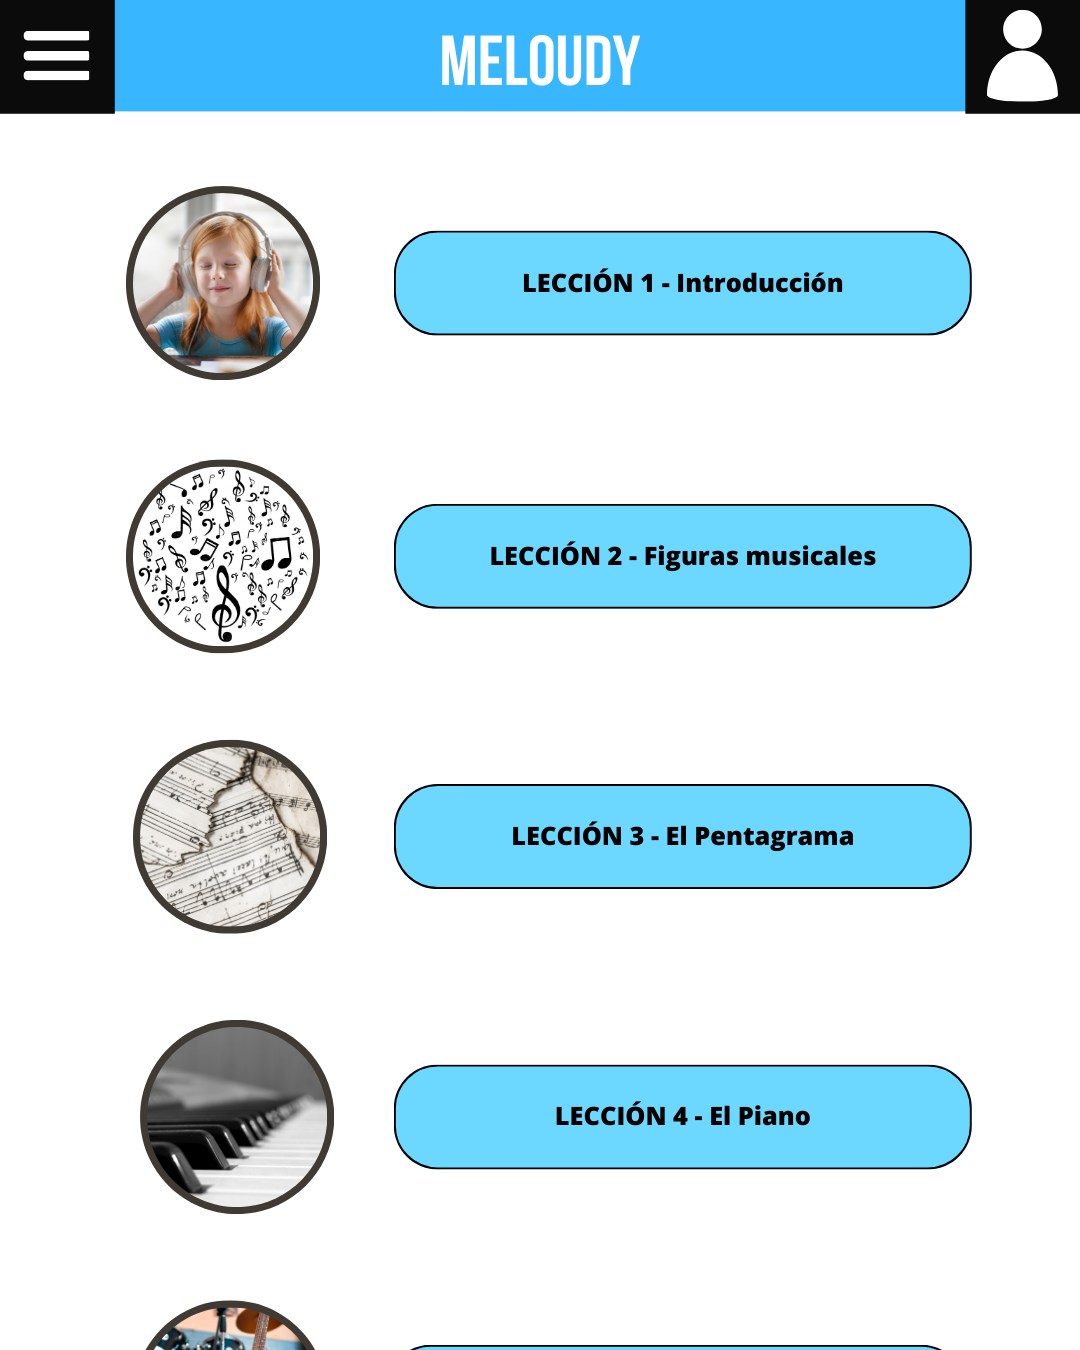
\includegraphics[width=0.8\textwidth]{imagenes/c3/boceto.png}
    \caption{Primer boceto de la interfaz de usuario de la página de inicio de la aplicación para los usuarios, donde se muestra la lista de las lecciones}
    \label{fig:artly}

\end{figure}